% This generates the PA DAWG presentation for a quarter of data
% 
% Copyright 2017 United States Government as represented by the
% Administrator of the National Aeronautics and Space Administration.
% All Rights Reserved.
% 
% This file is available under the terms of the NASA Open Source Agreement
% (NOSA). You should have received a copy of this agreement with the
% Kepler source code; see the file NASA-OPEN-SOURCE-AGREEMENT.doc.
% 
% No Warranty: THE SUBJECT SOFTWARE IS PROVIDED "AS IS" WITHOUT ANY
% WARRANTY OF ANY KIND, EITHER EXPRESSED, IMPLIED, OR STATUTORY,
% INCLUDING, BUT NOT LIMITED TO, ANY WARRANTY THAT THE SUBJECT SOFTWARE
% WILL CONFORM TO SPECIFICATIONS, ANY IMPLIED WARRANTIES OF
% MERCHANTABILITY, FITNESS FOR A PARTICULAR PURPOSE, OR FREEDOM FROM
% INFRINGEMENT, ANY WARRANTY THAT THE SUBJECT SOFTWARE WILL BE ERROR
% FREE, OR ANY WARRANTY THAT DOCUMENTATION, IF PROVIDED, WILL CONFORM
% TO THE SUBJECT SOFTWARE. THIS AGREEMENT DOES NOT, IN ANY MANNER,
% CONSTITUTE AN ENDORSEMENT BY GOVERNMENT AGENCY OR ANY PRIOR RECIPIENT
% OF ANY RESULTS, RESULTING DESIGNS, HARDWARE, SOFTWARE PRODUCTS OR ANY
% OTHER APPLICATIONS RESULTING FROM USE OF THE SUBJECT SOFTWARE.
% FURTHER, GOVERNMENT AGENCY DISCLAIMS ALL WARRANTIES AND LIABILITIES
% REGARDING THIRD-PARTY SOFTWARE, IF PRESENT IN THE ORIGINAL SOFTWARE,
% AND DISTRIBUTES IT "AS IS."
%
% Waiver and Indemnity: RECIPIENT AGREES TO WAIVE ANY AND ALL CLAIMS
% AGAINST THE UNITED STATES GOVERNMENT, ITS CONTRACTORS AND
% SUBCONTRACTORS, AS WELL AS ANY PRIOR RECIPIENT. IF RECIPIENT'S USE OF
% THE SUBJECT SOFTWARE RESULTS IN ANY LIABILITIES, DEMANDS, DAMAGES,
% EXPENSES OR LOSSES ARISING FROM SUCH USE, INCLUDING ANY DAMAGES FROM
% PRODUCTS BASED ON, OR RESULTING FROM, RECIPIENT'S USE OF THE SUBJECT
% SOFTWARE, RECIPIENT SHALL INDEMNIFY AND HOLD HARMLESS THE UNITED
% STATES GOVERNMENT, ITS CONTRACTORS AND SUBCONTRACTORS, AS WELL AS ANY
% PRIOR RECIPIENT, TO THE EXTENT PERMITTED BY LAW. RECIPIENT'S SOLE
% REMEDY FOR ANY SUCH MATTER SHALL BE THE IMMEDIATE, UNILATERAL
% TERMINATION OF THIS AGREEMENT.
%

\documentclass{article}

\usepackage[landscape]{geometry}
\usepackage{dawgpresentation}
\usepackage{report-definitions}
\usepackage{report-inputs}
\usepackage{scalefnt}
\usepackage{subfigure}
\usepackage{amsfonts}

\usepackage[pdftex]{graphicx} % must come before epstopdf
\usepackage{epstopdf}
\graphicspath{\reportgraphicspath}

\begin{document}

\scalefont{1.5}

%%%%%%%%%%%%%%%%%%%%%%%%%%%% TITLE SLIDE %%%%%%%%%%%%%%%%%%%%%%%%%%%%%%

% Title slide for DAWG presentation
% 
% Copyright 2017 United States Government as represented by the
% Administrator of the National Aeronautics and Space Administration.
% All Rights Reserved.
% 
% This file is available under the terms of the NASA Open Source Agreement
% (NOSA). You should have received a copy of this agreement with the
% Kepler source code; see the file NASA-OPEN-SOURCE-AGREEMENT.doc.
% 
% No Warranty: THE SUBJECT SOFTWARE IS PROVIDED "AS IS" WITHOUT ANY
% WARRANTY OF ANY KIND, EITHER EXPRESSED, IMPLIED, OR STATUTORY,
% INCLUDING, BUT NOT LIMITED TO, ANY WARRANTY THAT THE SUBJECT SOFTWARE
% WILL CONFORM TO SPECIFICATIONS, ANY IMPLIED WARRANTIES OF
% MERCHANTABILITY, FITNESS FOR A PARTICULAR PURPOSE, OR FREEDOM FROM
% INFRINGEMENT, ANY WARRANTY THAT THE SUBJECT SOFTWARE WILL BE ERROR
% FREE, OR ANY WARRANTY THAT DOCUMENTATION, IF PROVIDED, WILL CONFORM
% TO THE SUBJECT SOFTWARE. THIS AGREEMENT DOES NOT, IN ANY MANNER,
% CONSTITUTE AN ENDORSEMENT BY GOVERNMENT AGENCY OR ANY PRIOR RECIPIENT
% OF ANY RESULTS, RESULTING DESIGNS, HARDWARE, SOFTWARE PRODUCTS OR ANY
% OTHER APPLICATIONS RESULTING FROM USE OF THE SUBJECT SOFTWARE.
% FURTHER, GOVERNMENT AGENCY DISCLAIMS ALL WARRANTIES AND LIABILITIES
% REGARDING THIRD-PARTY SOFTWARE, IF PRESENT IN THE ORIGINAL SOFTWARE,
% AND DISTRIBUTES IT "AS IS."
%
% Waiver and Indemnity: RECIPIENT AGREES TO WAIVE ANY AND ALL CLAIMS
% AGAINST THE UNITED STATES GOVERNMENT, ITS CONTRACTORS AND
% SUBCONTRACTORS, AS WELL AS ANY PRIOR RECIPIENT. IF RECIPIENT'S USE OF
% THE SUBJECT SOFTWARE RESULTS IN ANY LIABILITIES, DEMANDS, DAMAGES,
% EXPENSES OR LOSSES ARISING FROM SUCH USE, INCLUDING ANY DAMAGES FROM
% PRODUCTS BASED ON, OR RESULTING FROM, RECIPIENT'S USE OF THE SUBJECT
% SOFTWARE, RECIPIENT SHALL INDEMNIFY AND HOLD HARMLESS THE UNITED
% STATES GOVERNMENT, ITS CONTRACTORS AND SUBCONTRACTORS, AS WELL AS ANY
% PRIOR RECIPIENT, TO THE EXTENT PERMITTED BY LAW. RECIPIENT'S SOLE
% REMEDY FOR ANY SUCH MATTER SHALL BE THE IMMEDIATE, UNILATERAL
% TERMINATION OF THIS AGREEMENT.
%

\begin{center}

\begin{figure*}[h!]
\subfigure{\includegraphics[width=2in]{\logo}}
\hfill
\subfigure{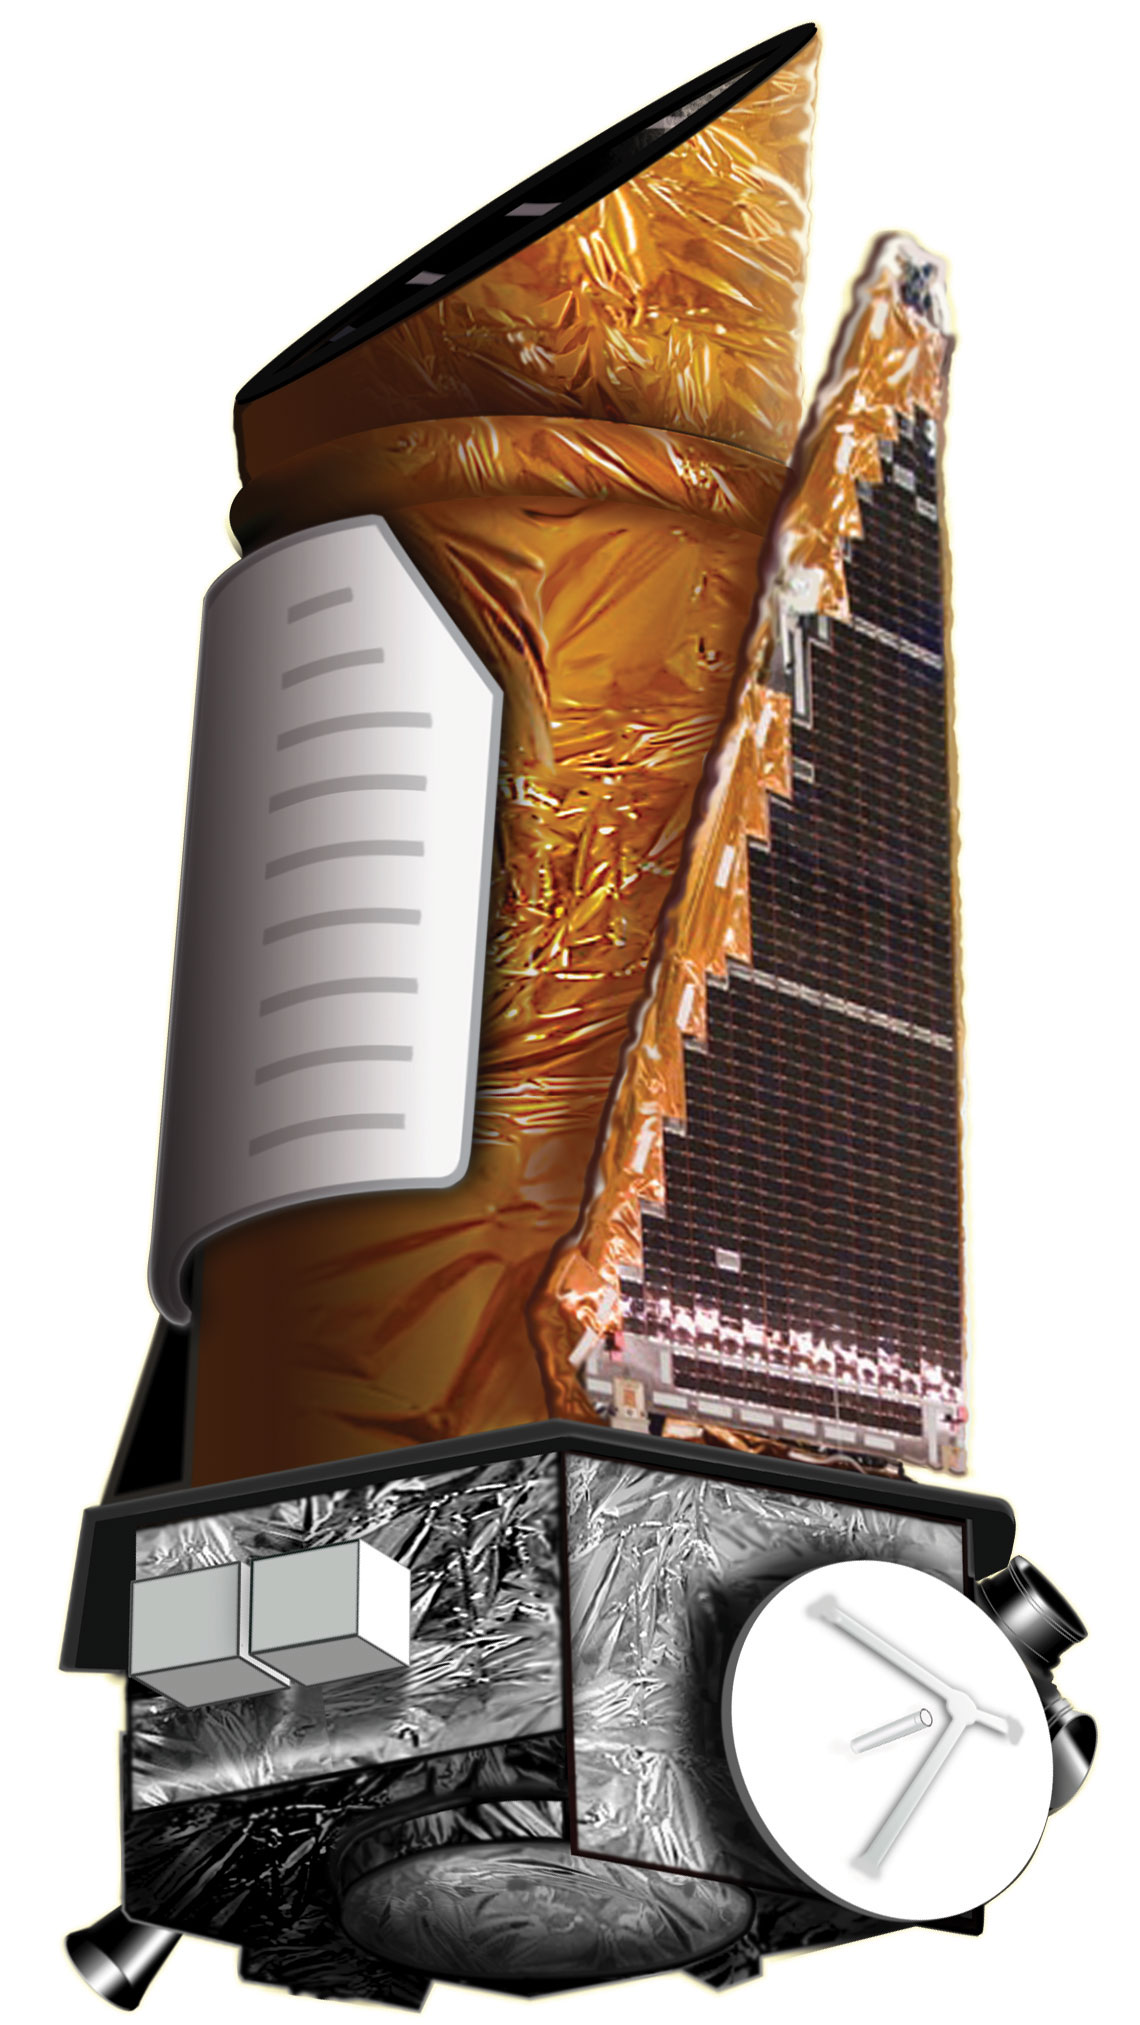
\includegraphics[angle=45,width=1in]{Kepler_spacecraft.png}}
\end{figure*}

\hrule

\vspace{2in}

{\Huge {\bf PA \swversion\ DAWG REVIEW FOR Q0-Q17 LC}}

\vspace{1in}

{\huge Generated \today}
\end{center}


%%%%%%%%%%%%%%%%%%%% CONTENTS SUMMARY SLIDE %%%%%%%%%%%%%%%%%%%%%%%%%

\newcommand{\slideTitle}{{\Huge {\bf PA \quarter\ SC Data}}}
%
% Copyright 2017 United States Government as represented by the
% Administrator of the National Aeronautics and Space Administration.
% All Rights Reserved.
% 
% This file is available under the terms of the NASA Open Source Agreement
% (NOSA). You should have received a copy of this agreement with the
% Kepler source code; see the file NASA-OPEN-SOURCE-AGREEMENT.doc.
% 
% No Warranty: THE SUBJECT SOFTWARE IS PROVIDED "AS IS" WITHOUT ANY
% WARRANTY OF ANY KIND, EITHER EXPRESSED, IMPLIED, OR STATUTORY,
% INCLUDING, BUT NOT LIMITED TO, ANY WARRANTY THAT THE SUBJECT SOFTWARE
% WILL CONFORM TO SPECIFICATIONS, ANY IMPLIED WARRANTIES OF
% MERCHANTABILITY, FITNESS FOR A PARTICULAR PURPOSE, OR FREEDOM FROM
% INFRINGEMENT, ANY WARRANTY THAT THE SUBJECT SOFTWARE WILL BE ERROR
% FREE, OR ANY WARRANTY THAT DOCUMENTATION, IF PROVIDED, WILL CONFORM
% TO THE SUBJECT SOFTWARE. THIS AGREEMENT DOES NOT, IN ANY MANNER,
% CONSTITUTE AN ENDORSEMENT BY GOVERNMENT AGENCY OR ANY PRIOR RECIPIENT
% OF ANY RESULTS, RESULTING DESIGNS, HARDWARE, SOFTWARE PRODUCTS OR ANY
% OTHER APPLICATIONS RESULTING FROM USE OF THE SUBJECT SOFTWARE.
% FURTHER, GOVERNMENT AGENCY DISCLAIMS ALL WARRANTIES AND LIABILITIES
% REGARDING THIRD-PARTY SOFTWARE, IF PRESENT IN THE ORIGINAL SOFTWARE,
% AND DISTRIBUTES IT "AS IS."
%
% Waiver and Indemnity: RECIPIENT AGREES TO WAIVE ANY AND ALL CLAIMS
% AGAINST THE UNITED STATES GOVERNMENT, ITS CONTRACTORS AND
% SUBCONTRACTORS, AS WELL AS ANY PRIOR RECIPIENT. IF RECIPIENT'S USE OF
% THE SUBJECT SOFTWARE RESULTS IN ANY LIABILITIES, DEMANDS, DAMAGES,
% EXPENSES OR LOSSES ARISING FROM SUCH USE, INCLUDING ANY DAMAGES FROM
% PRODUCTS BASED ON, OR RESULTING FROM, RECIPIENT'S USE OF THE SUBJECT
% SOFTWARE, RECIPIENT SHALL INDEMNIFY AND HOLD HARMLESS THE UNITED
% STATES GOVERNMENT, ITS CONTRACTORS AND SUBCONTRACTORS, AS WELL AS ANY
% PRIOR RECIPIENT, TO THE EXTENT PERMITTED BY LAW. RECIPIENT'S SOLE
% REMEDY FOR ANY SUCH MATTER SHALL BE THE IMMEDIATE, UNILATERAL
% TERMINATION OF THIS AGREEMENT.
%
\cleardoublepage
\begin{figure*}[h!]
  \centering
  \subfigure{\includegraphics[width=1in]{\logo}}
  \hfill
  \slideTitle
  \hfill
  \subfigure{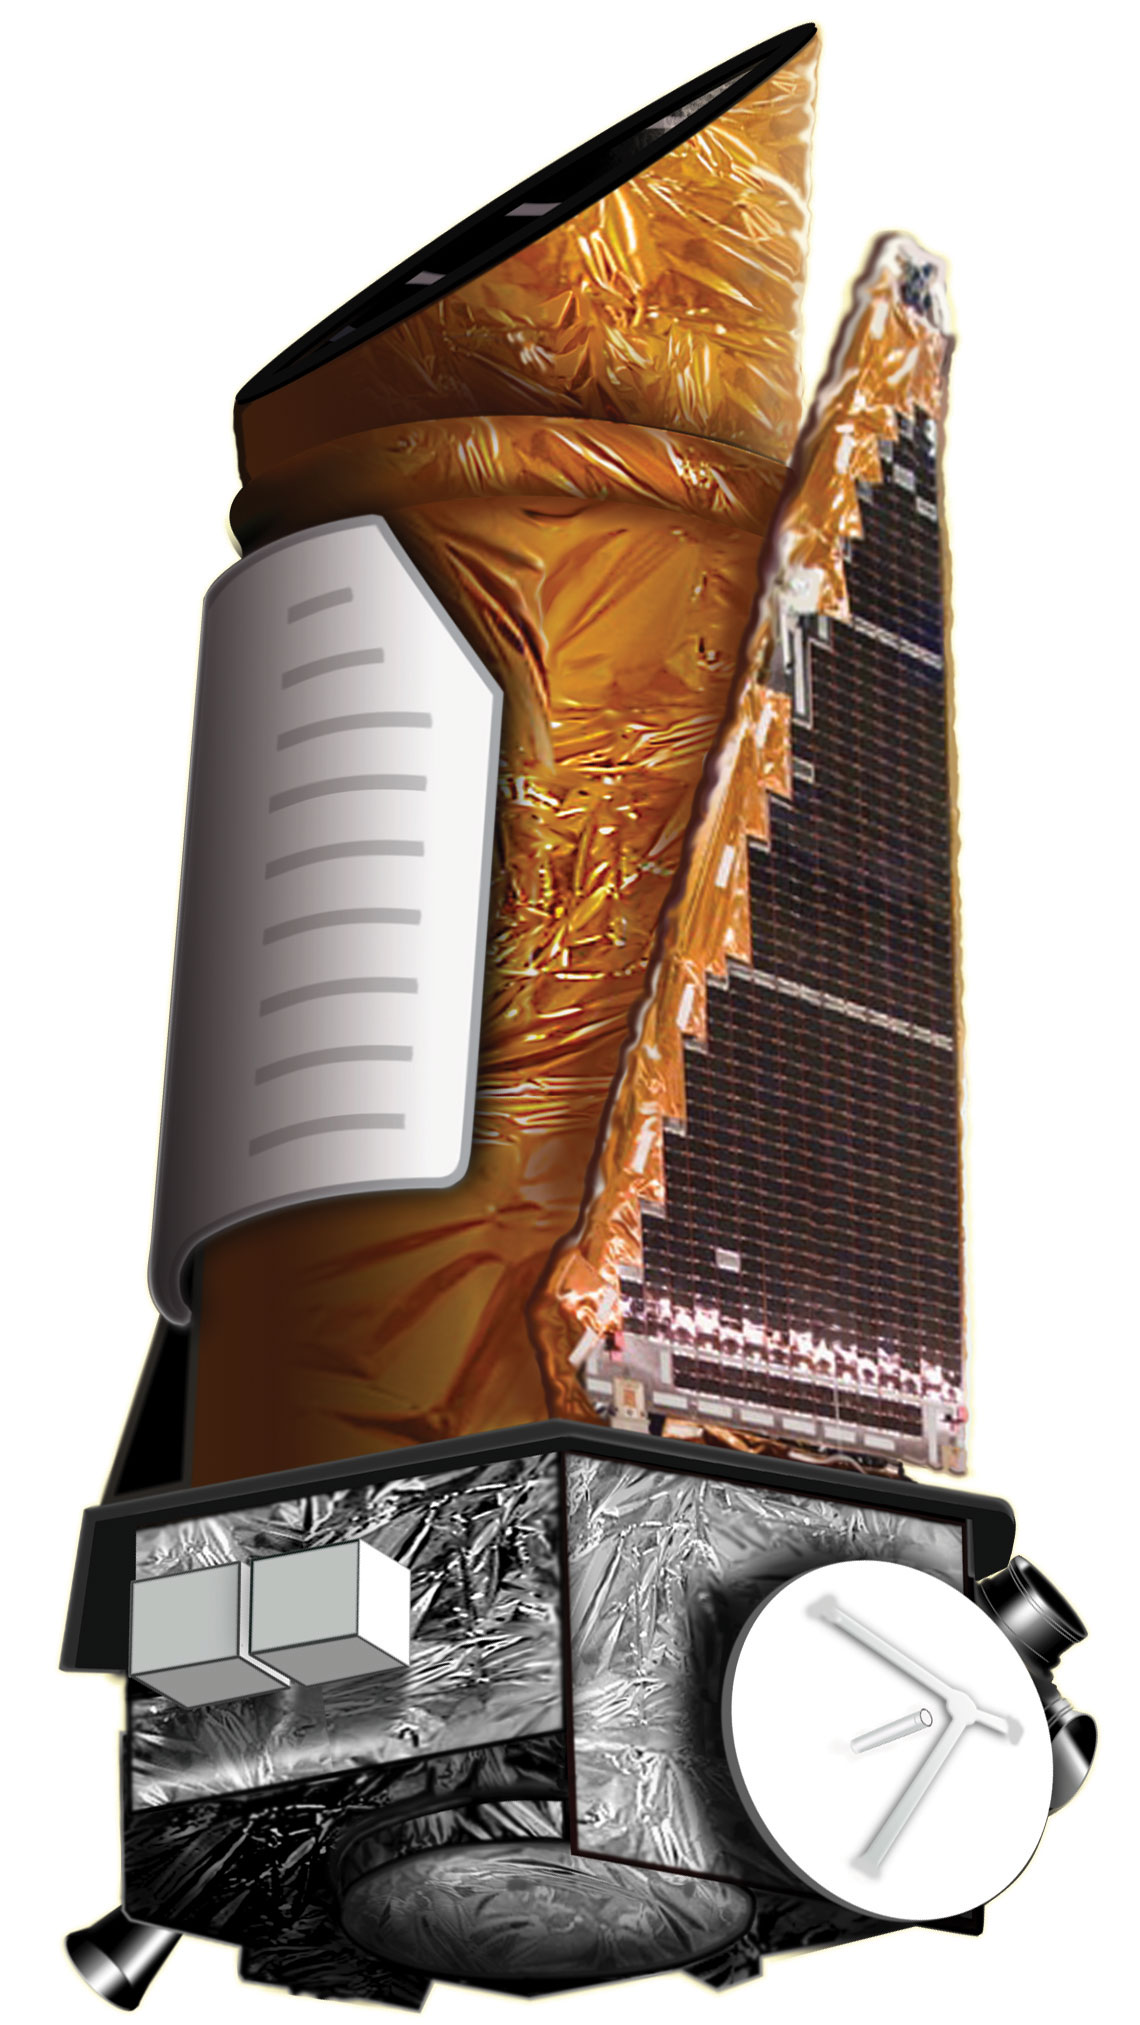
\includegraphics[angle=45,width=1in]{Kepler_spacecraft.png}}
\end{figure*}
\hrule

% Slide for the DAWG presentation intro
% 
% Copyright 2017 United States Government as represented by the
% Administrator of the National Aeronautics and Space Administration.
% All Rights Reserved.
% 
% This file is available under the terms of the NASA Open Source Agreement
% (NOSA). You should have received a copy of this agreement with the
% Kepler source code; see the file NASA-OPEN-SOURCE-AGREEMENT.doc.
% 
% No Warranty: THE SUBJECT SOFTWARE IS PROVIDED "AS IS" WITHOUT ANY
% WARRANTY OF ANY KIND, EITHER EXPRESSED, IMPLIED, OR STATUTORY,
% INCLUDING, BUT NOT LIMITED TO, ANY WARRANTY THAT THE SUBJECT SOFTWARE
% WILL CONFORM TO SPECIFICATIONS, ANY IMPLIED WARRANTIES OF
% MERCHANTABILITY, FITNESS FOR A PARTICULAR PURPOSE, OR FREEDOM FROM
% INFRINGEMENT, ANY WARRANTY THAT THE SUBJECT SOFTWARE WILL BE ERROR
% FREE, OR ANY WARRANTY THAT DOCUMENTATION, IF PROVIDED, WILL CONFORM
% TO THE SUBJECT SOFTWARE. THIS AGREEMENT DOES NOT, IN ANY MANNER,
% CONSTITUTE AN ENDORSEMENT BY GOVERNMENT AGENCY OR ANY PRIOR RECIPIENT
% OF ANY RESULTS, RESULTING DESIGNS, HARDWARE, SOFTWARE PRODUCTS OR ANY
% OTHER APPLICATIONS RESULTING FROM USE OF THE SUBJECT SOFTWARE.
% FURTHER, GOVERNMENT AGENCY DISCLAIMS ALL WARRANTIES AND LIABILITIES
% REGARDING THIRD-PARTY SOFTWARE, IF PRESENT IN THE ORIGINAL SOFTWARE,
% AND DISTRIBUTES IT "AS IS."
%
% Waiver and Indemnity: RECIPIENT AGREES TO WAIVE ANY AND ALL CLAIMS
% AGAINST THE UNITED STATES GOVERNMENT, ITS CONTRACTORS AND
% SUBCONTRACTORS, AS WELL AS ANY PRIOR RECIPIENT. IF RECIPIENT'S USE OF
% THE SUBJECT SOFTWARE RESULTS IN ANY LIABILITIES, DEMANDS, DAMAGES,
% EXPENSES OR LOSSES ARISING FROM SUCH USE, INCLUDING ANY DAMAGES FROM
% PRODUCTS BASED ON, OR RESULTING FROM, RECIPIENT'S USE OF THE SUBJECT
% SOFTWARE, RECIPIENT SHALL INDEMNIFY AND HOLD HARMLESS THE UNITED
% STATES GOVERNMENT, ITS CONTRACTORS AND SUBCONTRACTORS, AS WELL AS ANY
% PRIOR RECIPIENT, TO THE EXTENT PERMITTED BY LAW. RECIPIENT'S SOLE
% REMEDY FOR ANY SUCH MATTER SHALL BE THE IMMEDIATE, UNILATERAL
% TERMINATION OF THIS AGREEMENT.
%
\begin{itemize}

\item Examine long cadence CSCI outputs

  \begin{itemize}
    \item Background polynomial fits
    \item Motion polynomial fits
    \item Raw flux time series including PA-COA metrics
    \item Centroid time series
    \item Detected Cosmic Ray Distribution
    \item Argabrightenings and Reaction wheel zero crossings
  \end{itemize}

%\item Examine short cadence CSCI outputs
%
%  \begin{itemize}
%    \item Raw flux time series
%    \item Centroid time series
%  \end{itemize}

\end{itemize}


%%%%%%%%%%%%%%%%% START THE SC SET OF SLIDES %%%%%%%%%%%%%%%%%%%%%%%%

%%START SLIDE 
% 
% Copyright 2017 United States Government as represented by the
% Administrator of the National Aeronautics and Space Administration.
% All Rights Reserved.
% 
% This file is available under the terms of the NASA Open Source Agreement
% (NOSA). You should have received a copy of this agreement with the
% Kepler source code; see the file NASA-OPEN-SOURCE-AGREEMENT.doc.
% 
% No Warranty: THE SUBJECT SOFTWARE IS PROVIDED "AS IS" WITHOUT ANY
% WARRANTY OF ANY KIND, EITHER EXPRESSED, IMPLIED, OR STATUTORY,
% INCLUDING, BUT NOT LIMITED TO, ANY WARRANTY THAT THE SUBJECT SOFTWARE
% WILL CONFORM TO SPECIFICATIONS, ANY IMPLIED WARRANTIES OF
% MERCHANTABILITY, FITNESS FOR A PARTICULAR PURPOSE, OR FREEDOM FROM
% INFRINGEMENT, ANY WARRANTY THAT THE SUBJECT SOFTWARE WILL BE ERROR
% FREE, OR ANY WARRANTY THAT DOCUMENTATION, IF PROVIDED, WILL CONFORM
% TO THE SUBJECT SOFTWARE. THIS AGREEMENT DOES NOT, IN ANY MANNER,
% CONSTITUTE AN ENDORSEMENT BY GOVERNMENT AGENCY OR ANY PRIOR RECIPIENT
% OF ANY RESULTS, RESULTING DESIGNS, HARDWARE, SOFTWARE PRODUCTS OR ANY
% OTHER APPLICATIONS RESULTING FROM USE OF THE SUBJECT SOFTWARE.
% FURTHER, GOVERNMENT AGENCY DISCLAIMS ALL WARRANTIES AND LIABILITIES
% REGARDING THIRD-PARTY SOFTWARE, IF PRESENT IN THE ORIGINAL SOFTWARE,
% AND DISTRIBUTES IT "AS IS."
%
% Waiver and Indemnity: RECIPIENT AGREES TO WAIVE ANY AND ALL CLAIMS
% AGAINST THE UNITED STATES GOVERNMENT, ITS CONTRACTORS AND
% SUBCONTRACTORS, AS WELL AS ANY PRIOR RECIPIENT. IF RECIPIENT'S USE OF
% THE SUBJECT SOFTWARE RESULTS IN ANY LIABILITIES, DEMANDS, DAMAGES,
% EXPENSES OR LOSSES ARISING FROM SUCH USE, INCLUDING ANY DAMAGES FROM
% PRODUCTS BASED ON, OR RESULTING FROM, RECIPIENT'S USE OF THE SUBJECT
% SOFTWARE, RECIPIENT SHALL INDEMNIFY AND HOLD HARMLESS THE UNITED
% STATES GOVERNMENT, ITS CONTRACTORS AND SUBCONTRACTORS, AS WELL AS ANY
% PRIOR RECIPIENT, TO THE EXTENT PERMITTED BY LAW. RECIPIENT'S SOLE
% REMEDY FOR ANY SUCH MATTER SHALL BE THE IMMEDIATE, UNILATERAL
% TERMINATION OF THIS AGREEMENT.
%
\cleardoublepage
\begin{figure*}[h!]
  \centering
  \subfigure{\includegraphics[width=1in]{\logo}}
  \hfill
  \hfill
  \subfigure{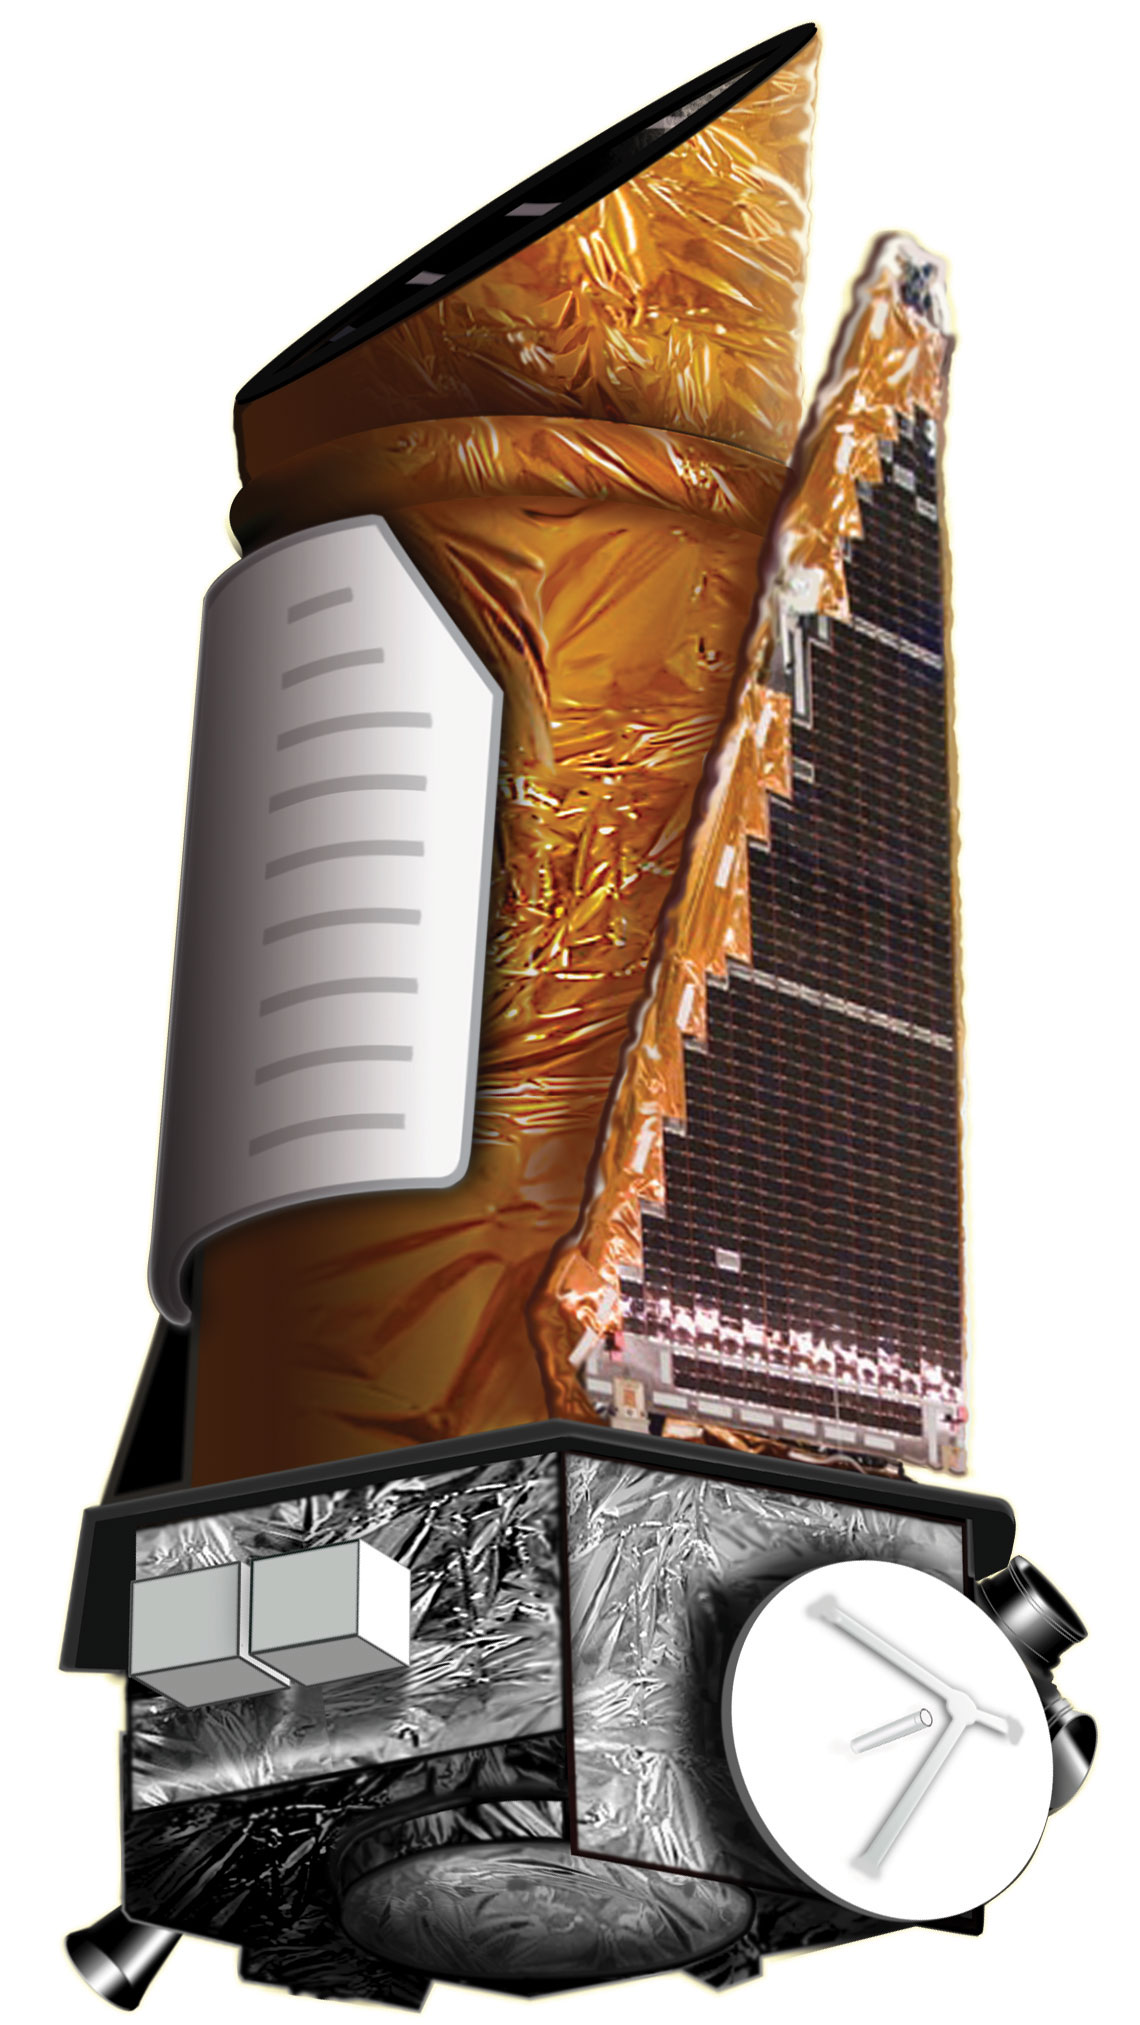
\includegraphics[angle=45,width=1in]{Kepler_spacecraft.png}}
\end{figure*}
\hrule

%% END SLIDE 
\vspace{2in}
\centering
{\Huge {\bf \quarter\ SC Flux Time Series}}



%%START SLIDE 
\cleardoublepage
\begin{figure*}[h!]
  \centering
  \subfigure{\includegraphics[width=1in]{\logo}}
  \hfill
  {\Huge {\bf \quarter\ SC M1 Flux Distributions}}
  \hfill
  \subfigure{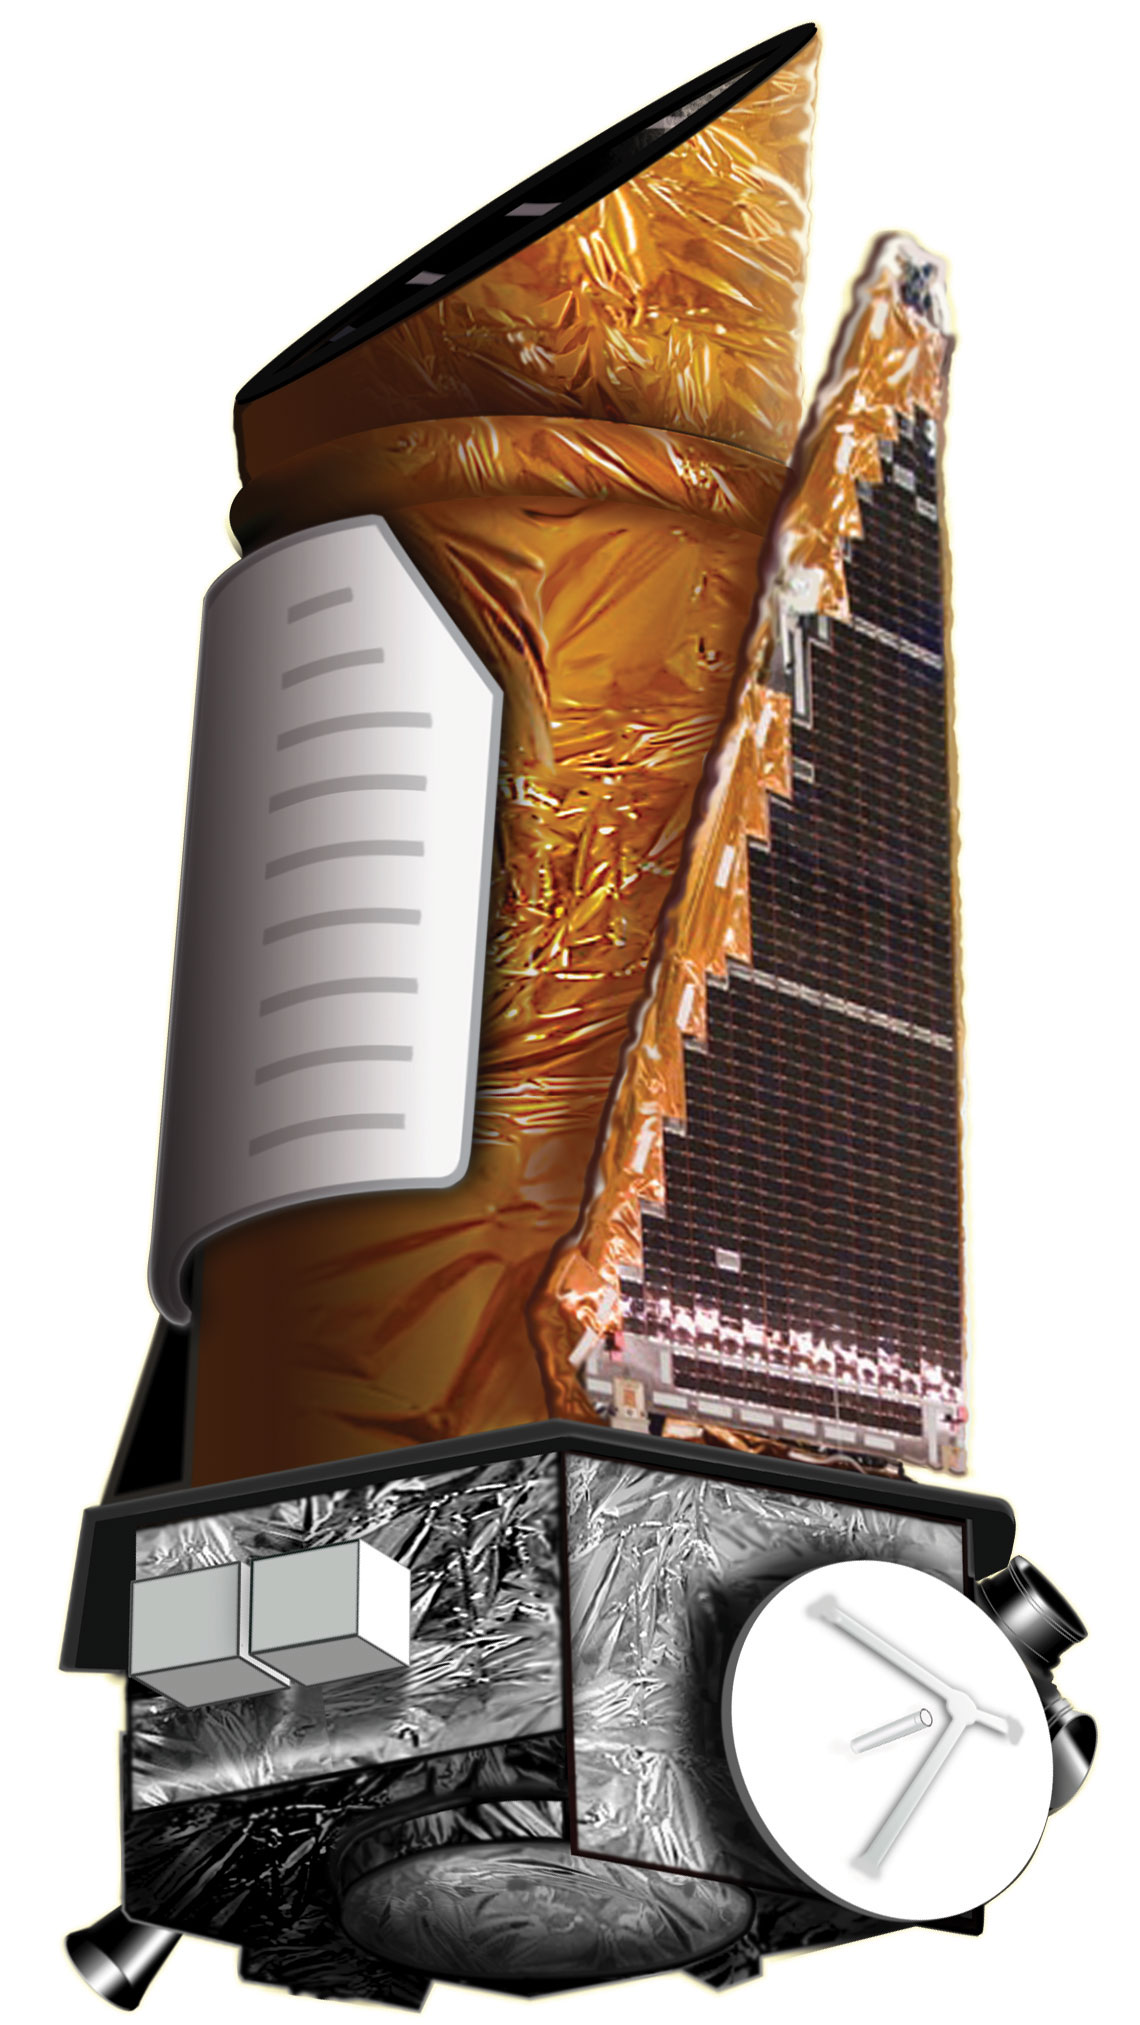
\includegraphics[angle=45,width=1in]{Kepler_spacecraft.png}}
\end{figure*}
\hrule

\begin{figure*}[h!]
  \centering
  \includegraphics[width=0.45\textwidth]{flux_figures/sc_m1/median_flux_over_expected_flux_dist.eps}
  \includegraphics[width=0.45\textwidth]{flux_figures/sc_m1/median_uncertainty_over_shot_noise_dist.eps}
  \caption{Left: Ratio of median flux to expected flux.  Right: Ratio of median flux standard deviation to shot noise}
\end{figure*}


%% END SLIDE 

%%%START SLIDE 
%\cleardoublepage
%\begin{figure*}[h!]
%  \centering
%  \subfigure{\includegraphics[width=1in]{\logo}}
%  \hfill
%  {\Huge {\bf \quarter\ SC M2 Flux Distributions}}
%  \hfill
%  \subfigure{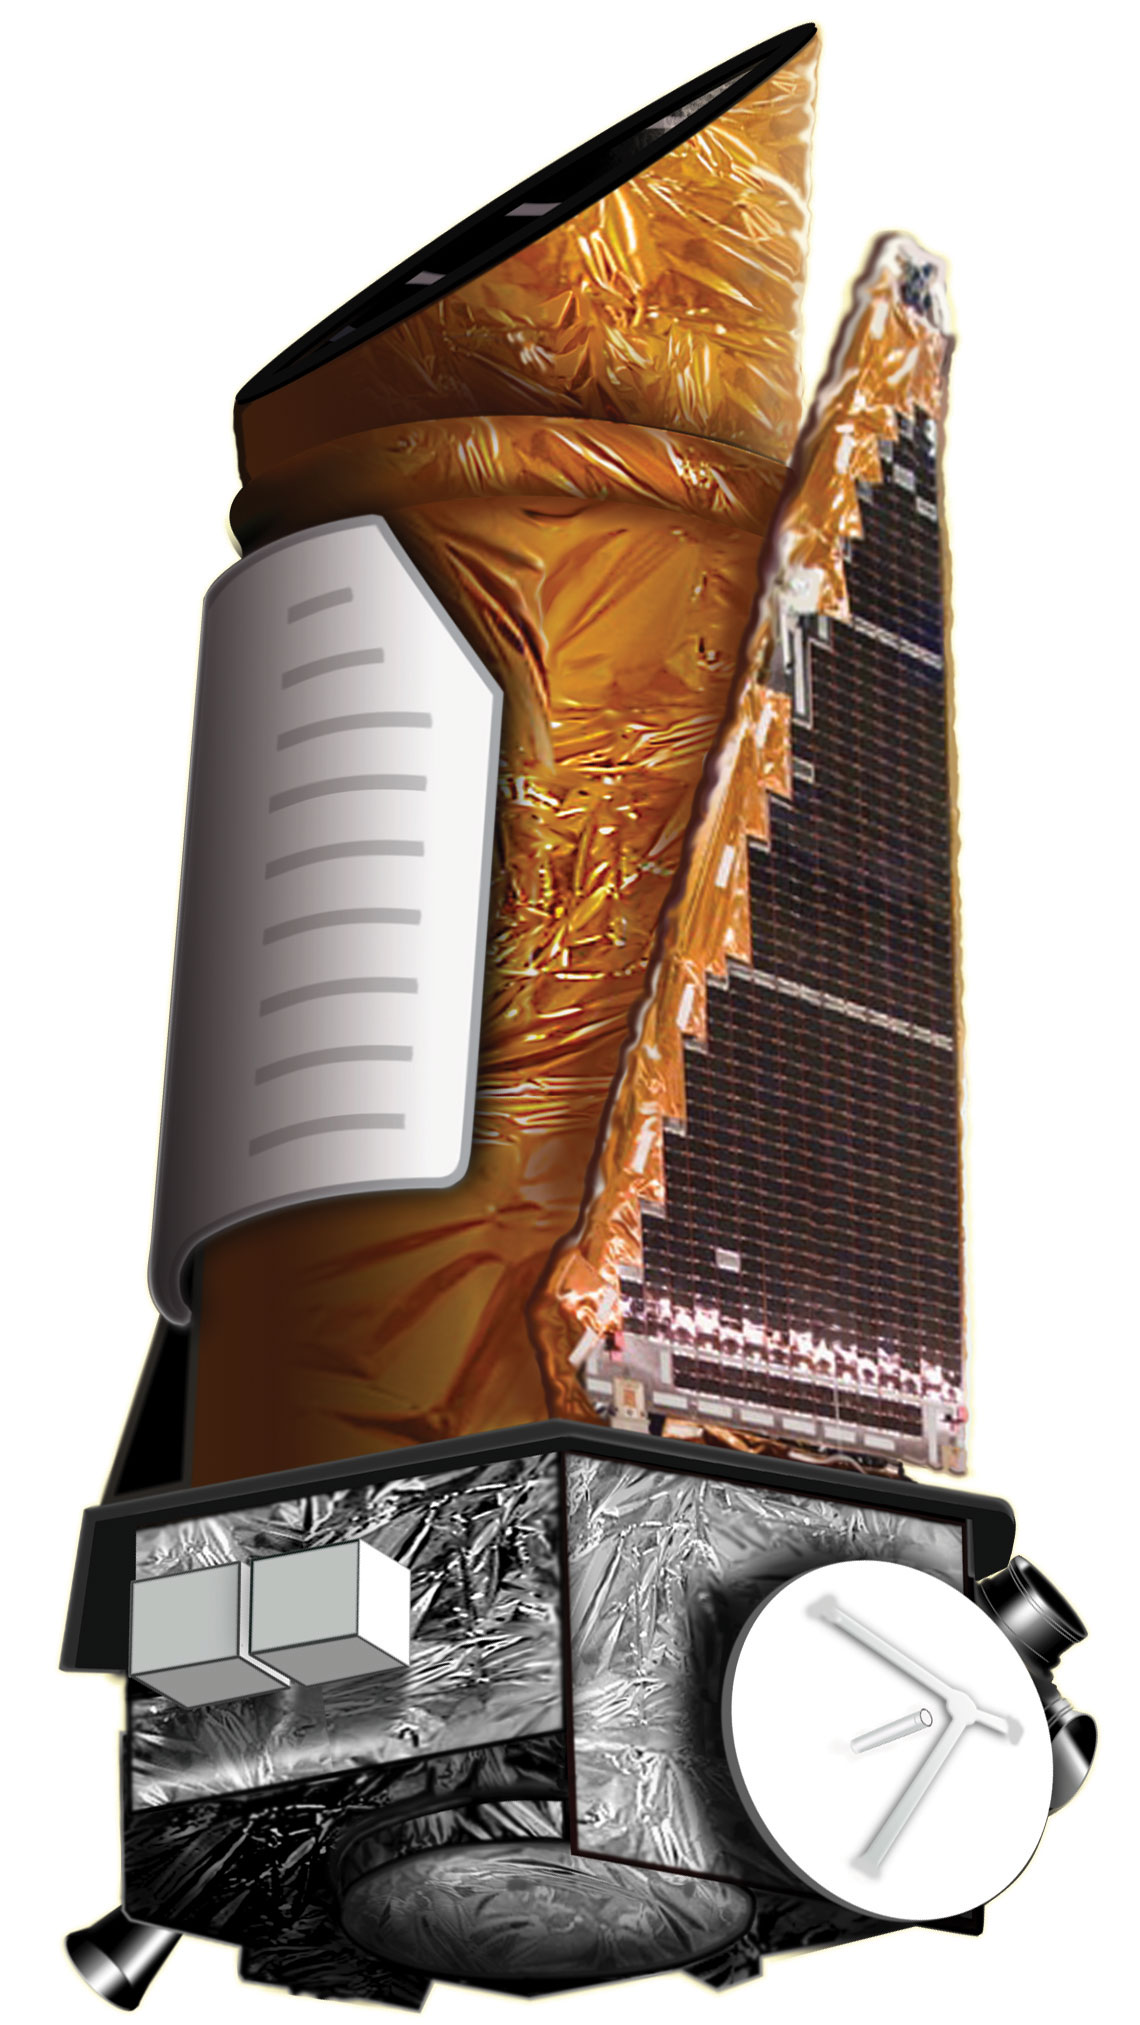
\includegraphics[angle=45,width=1in]{Kepler_spacecraft.png}}
%\end{figure*}
%\hrule
%
%\begin{figure*}[h!]
%  \centering
%  \includegraphics[width=0.45\textwidth]{flux_figures/sc_m2/median_flux_over_expected_flux_dist.eps}
%  \includegraphics[width=0.45\textwidth]{flux_figures/sc_m2/median_uncertainty_over_shot_noise_dist.eps}
%  \caption{Left: Ratio of median flux to expected flux.  Right: Ratio of median flux standard deviation to shot noise}
%\end{figure*}
%
%
%%% END SLIDE 
%
%%START SLIDE 
%\cleardoublepage
%\begin{figure*}[h!]
%  \centering
%  \subfigure{\includegraphics[width=1in]{\logo}}
%  \hfill
%  {\Huge {\bf \quarter\ SC M3 Flux Distributions}}
%  \hfill
%  \subfigure{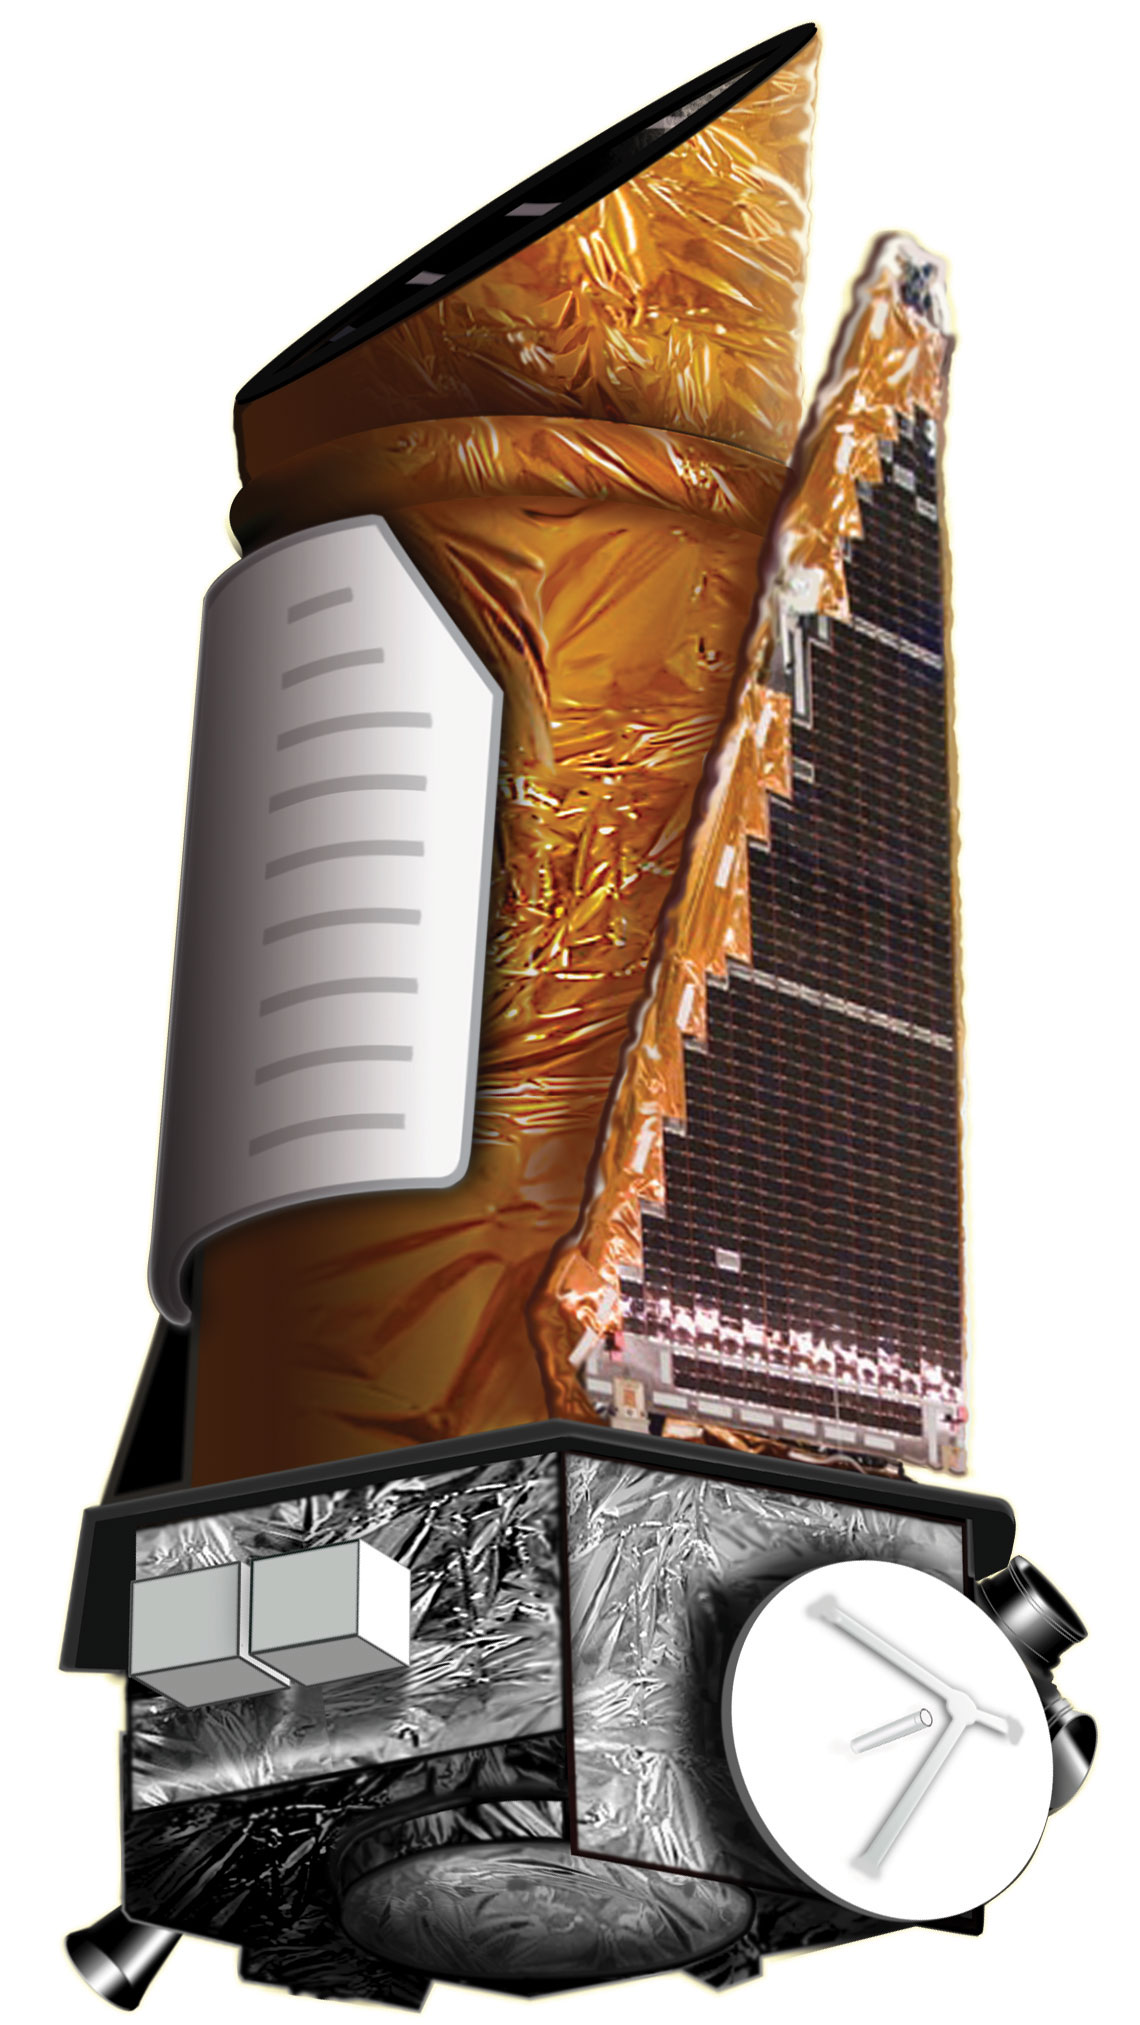
\includegraphics[angle=45,width=1in]{Kepler_spacecraft.png}}
%\end{figure*}
%\hrule
%
%\begin{figure*}[h!]
%  \centering
%  \includegraphics[width=0.45\textwidth]{flux_figures/sc_m3/median_flux_over_expected_flux_dist.eps}
%  \includegraphics[width=0.45\textwidth]{flux_figures/sc_m3/median_uncertainty_over_shot_noise_dist.eps}
%  \caption{Left: Ratio of median flux to expected flux.  Right: Ratio of median flux standard deviation to shot noise}
%\end{figure*}
%
%
%%% END SLIDE 
%

%
% Copyright 2017 United States Government as represented by the
% Administrator of the National Aeronautics and Space Administration.
% All Rights Reserved.
% 
% This file is available under the terms of the NASA Open Source Agreement
% (NOSA). You should have received a copy of this agreement with the
% Kepler source code; see the file NASA-OPEN-SOURCE-AGREEMENT.doc.
% 
% No Warranty: THE SUBJECT SOFTWARE IS PROVIDED "AS IS" WITHOUT ANY
% WARRANTY OF ANY KIND, EITHER EXPRESSED, IMPLIED, OR STATUTORY,
% INCLUDING, BUT NOT LIMITED TO, ANY WARRANTY THAT THE SUBJECT SOFTWARE
% WILL CONFORM TO SPECIFICATIONS, ANY IMPLIED WARRANTIES OF
% MERCHANTABILITY, FITNESS FOR A PARTICULAR PURPOSE, OR FREEDOM FROM
% INFRINGEMENT, ANY WARRANTY THAT THE SUBJECT SOFTWARE WILL BE ERROR
% FREE, OR ANY WARRANTY THAT DOCUMENTATION, IF PROVIDED, WILL CONFORM
% TO THE SUBJECT SOFTWARE. THIS AGREEMENT DOES NOT, IN ANY MANNER,
% CONSTITUTE AN ENDORSEMENT BY GOVERNMENT AGENCY OR ANY PRIOR RECIPIENT
% OF ANY RESULTS, RESULTING DESIGNS, HARDWARE, SOFTWARE PRODUCTS OR ANY
% OTHER APPLICATIONS RESULTING FROM USE OF THE SUBJECT SOFTWARE.
% FURTHER, GOVERNMENT AGENCY DISCLAIMS ALL WARRANTIES AND LIABILITIES
% REGARDING THIRD-PARTY SOFTWARE, IF PRESENT IN THE ORIGINAL SOFTWARE,
% AND DISTRIBUTES IT "AS IS."
%
% Waiver and Indemnity: RECIPIENT AGREES TO WAIVE ANY AND ALL CLAIMS
% AGAINST THE UNITED STATES GOVERNMENT, ITS CONTRACTORS AND
% SUBCONTRACTORS, AS WELL AS ANY PRIOR RECIPIENT. IF RECIPIENT'S USE OF
% THE SUBJECT SOFTWARE RESULTS IN ANY LIABILITIES, DEMANDS, DAMAGES,
% EXPENSES OR LOSSES ARISING FROM SUCH USE, INCLUDING ANY DAMAGES FROM
% PRODUCTS BASED ON, OR RESULTING FROM, RECIPIENT'S USE OF THE SUBJECT
% SOFTWARE, RECIPIENT SHALL INDEMNIFY AND HOLD HARMLESS THE UNITED
% STATES GOVERNMENT, ITS CONTRACTORS AND SUBCONTRACTORS, AS WELL AS ANY
% PRIOR RECIPIENT, TO THE EXTENT PERMITTED BY LAW. RECIPIENT'S SOLE
% REMEDY FOR ANY SUCH MATTER SHALL BE THE IMMEDIATE, UNILATERAL
% TERMINATION OF THIS AGREEMENT.
%


%%%%%%%%%%%%%%%% END STANDARD SLIDES %%%%%%%%%%%%%%%%%%%%%%
%% Slide for the summary at the end of the DAWG presentation
% 
% Copyright 2017 United States Government as represented by the
% Administrator of the National Aeronautics and Space Administration.
% All Rights Reserved.
% 
% NASA acknowledges the SETI Institute's primary role in authoring and
% producing the Kepler Data Processing Pipeline under Cooperative
% Agreement Nos. NNA04CC63A, NNX07AD96A, NNX07AD98A, NNX11AI13A,
% NNX11AI14A, NNX13AD01A & NNX13AD16A.
% 
% This file is available under the terms of the NASA Open Source Agreement
% (NOSA). You should have received a copy of this agreement with the
% Kepler source code; see the file NASA-OPEN-SOURCE-AGREEMENT.doc.
% 
% No Warranty: THE SUBJECT SOFTWARE IS PROVIDED "AS IS" WITHOUT ANY
% WARRANTY OF ANY KIND, EITHER EXPRESSED, IMPLIED, OR STATUTORY,
% INCLUDING, BUT NOT LIMITED TO, ANY WARRANTY THAT THE SUBJECT SOFTWARE
% WILL CONFORM TO SPECIFICATIONS, ANY IMPLIED WARRANTIES OF
% MERCHANTABILITY, FITNESS FOR A PARTICULAR PURPOSE, OR FREEDOM FROM
% INFRINGEMENT, ANY WARRANTY THAT THE SUBJECT SOFTWARE WILL BE ERROR
% FREE, OR ANY WARRANTY THAT DOCUMENTATION, IF PROVIDED, WILL CONFORM
% TO THE SUBJECT SOFTWARE. THIS AGREEMENT DOES NOT, IN ANY MANNER,
% CONSTITUTE AN ENDORSEMENT BY GOVERNMENT AGENCY OR ANY PRIOR RECIPIENT
% OF ANY RESULTS, RESULTING DESIGNS, HARDWARE, SOFTWARE PRODUCTS OR ANY
% OTHER APPLICATIONS RESULTING FROM USE OF THE SUBJECT SOFTWARE.
% FURTHER, GOVERNMENT AGENCY DISCLAIMS ALL WARRANTIES AND LIABILITIES
% REGARDING THIRD-PARTY SOFTWARE, IF PRESENT IN THE ORIGINAL SOFTWARE,
% AND DISTRIBUTES IT "AS IS."
% 
% Waiver and Indemnity: RECIPIENT AGREES TO WAIVE ANY AND ALL CLAIMS
% AGAINST THE UNITED STATES GOVERNMENT, ITS CONTRACTORS AND
% SUBCONTRACTORS, AS WELL AS ANY PRIOR RECIPIENT. IF RECIPIENT'S USE OF
% THE SUBJECT SOFTWARE RESULTS IN ANY LIABILITIES, DEMANDS, DAMAGES,
% EXPENSES OR LOSSES ARISING FROM SUCH USE, INCLUDING ANY DAMAGES FROM
% PRODUCTS BASED ON, OR RESULTING FROM, RECIPIENT'S USE OF THE SUBJECT
% SOFTWARE, RECIPIENT SHALL INDEMNIFY AND HOLD HARMLESS THE UNITED
% STATES GOVERNMENT, ITS CONTRACTORS AND SUBCONTRACTORS, AS WELL AS ANY
% PRIOR RECIPIENT, TO THE EXTENT PERMITTED BY LAW. RECIPIENT'S SOLE
% REMEDY FOR ANY SUCH MATTER SHALL BE THE IMMEDIATE, UNILATERAL
% TERMINATION OF THIS AGREEMENT.
%
\begin{itemize}
        \item \quarter\ flight data was reprocessed with CAL \swversion\ code
        \begin{itemize}
                \item we examined collateral data for all channels
                \item we examined collateral and photometric data for 5 select channels 
                \item we also looked at pixel time series across cadence boundaries (CAL invocations)
        \end{itemize}
        \item Improvements in CAL \swversion\ :
        \begin{itemize}               
                \item KSOC-1099: Chatter in background pixels has been addressed with the implementation of an improved 1D Black model.
                \item KSOC-1126: Bleeding columns algorithm has been updated to include a fixed map of columns to exclude in smear estimate calculation.
        \end{itemize}
        \item Issues identified:
        \begin{itemize}               
                \item ...
                \item ...
        \end{itemize}
\end{itemize}



\end{document}
